\documentclass[10pt, french]{article}

%% -----------------------------
%% Préambule
%% -----------------------------
% !TEX encoding = UTF-8 Unicode
% LaTeX Preamble
% Author : Gabriel Crépeault-Cauchon

% HOW-TO : copy-paste this file in the same directory as your .tex file, and add in your preamble the next command right after you have specified your documentclass : 
% % !TEX encoding = UTF-8 Unicode
% LaTeX Preamble
% Author : Gabriel Crépeault-Cauchon
% Last update : 15/10/2018

% HOW-TO : copy-paste this file in the same directory as your .tex file, and add in your preamble the next command right after you have specified your documentclass : 
% % !TEX encoding = UTF-8 Unicode
% LaTeX Preamble
% Author : Gabriel Crépeault-Cauchon
% Last update : 15/10/2018

% HOW-TO : copy-paste this file in the same directory as your .tex file, and add in your preamble the next command right after you have specified your documentclass : 
% \input{preambule_utf8.tex}
% ---------------------------------------------
% ---------------------------------------------
%% BEGINNING OF PREAMBLE
% Encoding packages
\usepackage[utf8]{inputenc}
\usepackage[T1]{fontenc}
\usepackage{babel}
\usepackage{lmodern}

% HYPERREF (URL's and Link options)
\usepackage{hyperref}
\hypersetup{colorlinks = true, urlcolor = blue, linkcolor = black}

% POLICY (choose one of them)
%	\usepackage{concrete}
%	\usepackage{mathpazo}
%	\usepackage{frcursive} %% permet d'écrire en lettres attachées
%	\usepackage{aeguill}
	\usepackage{mathptmx}
%	\usepackage{fourier} 

% MATHEMATICS CONFIGURATION
\usepackage{amsmath,amsthm,amssymb,latexsym,amsfonts}
\usepackage{empheq}
\usepackage{numprint}


% TCOLORBOX CONFIGURATION
\usepackage{tcolorbox}
\tcbuselibrary{xparse}
\tcbuselibrary{breakable}
%% Définition Boite pour exemple
\newcounter{ex}[section]
\DeclareTColorBox{exemple}{ o }% #1 parameter
{colframe=green!20!black,colback=green!5!white, % color of the box
breakable, pad at break*=0mm, % to split the box
before title = {\textbf{Exemple \stepcounter{ex} \arabic{chapter}.\arabic{section}.\arabic{ex} }},
IfValueTF = {#1}{title= {#1}}{title= \hphantom},
after title = {\large \hfill \faWrench}
}% conditionnal usage : if a title is specified, use it, else put "Exemple"

%% Définition boite pour définition
\newcounter{def}[section]
\DeclareTColorBox{definition}{ o }% #1 parameter
{colframe=blue!60!green,colback=blue!5!white, % color of the box
breakable, pad at break*=0mm, % to split the box
before title = {\textbf{Définition \stepcounter{def} \arabic{chapter}.\arabic{section}.\arabic{def} }},
title = {#1},
after title = {\large \hfill \faBook}
}


% Graphics and picture import Packages
\usepackage{graphicx}
\usepackage{pict2e}

% insert PDF package
\usepackage{pdfpages}

% Color package
\usepackage{color, soulutf8, colortbl}

% usefull shortcut for colored text
\newcommand{\orange}{\textcolor{orange}}
\newcommand{\red}{\textcolor{red}}
\newcommand{\cyan}{\textcolor{cyan}}
\newcommand{\blue}{\textcolor{blue}}
\newcommand{\green}{\textcolor{green}}
\newcommand{\purple}{\textcolor{magenta}}
\newcommand{\yellow}{\textcolor{yellow}}

% Custum enumerate & itemize Package
\usepackage{enumitem}
% Change default label for itemize
\renewcommand{\labelitemi}{\faAngleRight}

% Mathematics shortcut macros
\newcommand{\reels}{\mathbb{R}}
\newcommand{\entiers}{\mathbb{Z}}
\newcommand{\naturels}{\mathbb{N}}
\newcommand{\eval}{\biggr \rvert}
\usepackage{cancel}
\newcommand{\derivee}[1]{\frac{\partial}{\partial #1}}
\newcommand{\prob}[1]{\Pr \left( #1 \right)}
\newcommand{\esp}[1]{\mathrm{E} \left[ #1 \right]}
\newcommand{\variance}[1]{\mathrm{VaR} \left( #1 \right)}
\newcommand{\laplace}{\mathcal{L}}
\newcommand{\indic}[1]{\mathds{1}_{\{ #1 \}}}

% Matricial notation (with simple command \bm{•})
\usepackage{bm}


% To indicate equation number on a specific line in align environment
\newcommand\numberthis{\addtocounter{equation}{1}\tag{\theequation}}

% Actuarial notation package
\usepackage{actuarialsymbol}
\usepackage{actuarialangle}

% Other shortcut
\newcommand{\p}{\paragraph{}}
\newcommand{\n}{\newline}

% Special symbols package
\usepackage[tikz]{bclogo}
\usepackage{fontawesome}

%% END OF PREAMBLE
% ---------------------------------------------
% ---------------------------------------------
% ---------------------------------------------
% ---------------------------------------------
%% BEGINNING OF PREAMBLE
% Encoding packages
\usepackage[utf8]{inputenc}
\usepackage[T1]{fontenc}
\usepackage{babel}
\usepackage{lmodern}

% HYPERREF (URL's and Link options)
\usepackage{hyperref}
\hypersetup{colorlinks = true, urlcolor = blue, linkcolor = black}

% POLICY (choose one of them)
%	\usepackage{concrete}
%	\usepackage{mathpazo}
%	\usepackage{frcursive} %% permet d'écrire en lettres attachées
%	\usepackage{aeguill}
	\usepackage{mathptmx}
%	\usepackage{fourier} 

% MATHEMATICS CONFIGURATION
\usepackage{amsmath,amsthm,amssymb,latexsym,amsfonts}
\usepackage{empheq}
\usepackage{numprint}


% TCOLORBOX CONFIGURATION
\usepackage{tcolorbox}
\tcbuselibrary{xparse}
\tcbuselibrary{breakable}
%% Définition Boite pour exemple
\newcounter{ex}[section]
\DeclareTColorBox{exemple}{ o }% #1 parameter
{colframe=green!20!black,colback=green!5!white, % color of the box
breakable, pad at break*=0mm, % to split the box
before title = {\textbf{Exemple \stepcounter{ex} \arabic{chapter}.\arabic{section}.\arabic{ex} }},
IfValueTF = {#1}{title= {#1}}{title= \hphantom},
after title = {\large \hfill \faWrench}
}% conditionnal usage : if a title is specified, use it, else put "Exemple"

%% Définition boite pour définition
\newcounter{def}[section]
\DeclareTColorBox{definition}{ o }% #1 parameter
{colframe=blue!60!green,colback=blue!5!white, % color of the box
breakable, pad at break*=0mm, % to split the box
before title = {\textbf{Définition \stepcounter{def} \arabic{chapter}.\arabic{section}.\arabic{def} }},
title = {#1},
after title = {\large \hfill \faBook}
}


% Graphics and picture import Packages
\usepackage{graphicx}
\usepackage{pict2e}

% insert PDF package
\usepackage{pdfpages}

% Color package
\usepackage{color, soulutf8, colortbl}

% usefull shortcut for colored text
\newcommand{\orange}{\textcolor{orange}}
\newcommand{\red}{\textcolor{red}}
\newcommand{\cyan}{\textcolor{cyan}}
\newcommand{\blue}{\textcolor{blue}}
\newcommand{\green}{\textcolor{green}}
\newcommand{\purple}{\textcolor{magenta}}
\newcommand{\yellow}{\textcolor{yellow}}

% Custum enumerate & itemize Package
\usepackage{enumitem}
% Change default label for itemize
\renewcommand{\labelitemi}{\faAngleRight}

% Mathematics shortcut macros
\newcommand{\reels}{\mathbb{R}}
\newcommand{\entiers}{\mathbb{Z}}
\newcommand{\naturels}{\mathbb{N}}
\newcommand{\eval}{\biggr \rvert}
\usepackage{cancel}
\newcommand{\derivee}[1]{\frac{\partial}{\partial #1}}
\newcommand{\prob}[1]{\Pr \left( #1 \right)}
\newcommand{\esp}[1]{\mathrm{E} \left[ #1 \right]}
\newcommand{\variance}[1]{\mathrm{VaR} \left( #1 \right)}
\newcommand{\laplace}{\mathcal{L}}
\newcommand{\indic}[1]{\mathds{1}_{\{ #1 \}}}

% Matricial notation (with simple command \bm{•})
\usepackage{bm}


% To indicate equation number on a specific line in align environment
\newcommand\numberthis{\addtocounter{equation}{1}\tag{\theequation}}

% Actuarial notation package
\usepackage{actuarialsymbol}
\usepackage{actuarialangle}

% Other shortcut
\newcommand{\p}{\paragraph{}}
\newcommand{\n}{\newline}

% Special symbols package
\usepackage[tikz]{bclogo}
\usepackage{fontawesome}

%% END OF PREAMBLE
% ---------------------------------------------
% ---------------------------------------------
% ---------------------------------------------
% ---------------------------------------------

%% -----------------------------
%% Encoding packages
%% -----------------------------
\usepackage[utf8]{inputenc}
\usepackage[T1]{fontenc}
\usepackage{babel}
\usepackage{lmodern}

%% -----------------------------
%% Variable definition
%% -----------------------------
\def\cours{Mathématiques actuarielles IARD1}
\def\sigle{ACT-2005}
\def\session{Automne 2018}
\def\auteur{Gabriel Crépeault-Cauchon}
\def\BackgroundColor{gray!20!white}
\def\SectionColor{red!80!white}
\def\SubSectionColor{red!30!black}


%% -----------------------------
%% Margin and layout
%% -----------------------------
\usepackage[hmargin=1cm, vmargin=1.7cm]{geometry}
\usepackage{multicol}

%% -----------------------------
%% URL and links
%% -----------------------------
\usepackage{hyperref}
\hypersetup{colorlinks = true, urlcolor = gray!60!black, linkcolor = black}

%% -----------------------------
%% Document policy (uncomment only one)
%% -----------------------------
%	\usepackage{concrete}
	\usepackage{mathpazo}
%	\usepackage{frcursive} %% permet d'écrire en lettres attachées
%	\usepackage{aeguill}
%	\usepackage{mathptmx}
%	\usepackage{fourier} 

%% -----------------------------
%% Math configuration
%% -----------------------------
\usepackage{amsmath,amsthm,amssymb,latexsym,amsfonts}
\usepackage{empheq}
\usepackage{numprint}

% Mathematics shortcut
\newcommand{\reels}{\mathbb{R}}
\newcommand{\entiers}{\mathbb{Z}}
\newcommand{\naturels}{\mathbb{N}}
\newcommand{\eval}{\biggr \rvert}
\usepackage{cancel}
\newcommand{\derivee}[1]{\frac{\partial}{\partial #1}}
\newcommand{\prob}[1]{\Pr \left( #1 \right)}
\newcommand{\esp}[1]{E \left[ #1 \right]}
\newcommand{\laplace}{\mathcal{L}}

% To indicate equation number on a specific line in align environment
\newcommand\numberthis{\addtocounter{equation}{1}\tag{\theequation}}

% Actuarial notation package
\usepackage{actuarialsymbol}
\usepackage{actuarialangle}




%% -----------------------------
%% tcolorbox configuration
%% -----------------------------
\usepackage{tcolorbox}
\tcbuselibrary{xparse}
\tcbuselibrary{breakable}

%% Définition boite pour définition
\DeclareTColorBox{definition}{ o }% #1 parameter
{colframe=blue!60!green,colback=blue!5!white, % color of the box
breakable, pad at break*=0mm, % to split the box
title = {#1},
after title = {\large \hfill \faBook}
}

%% -----------------------------
%% Graphics and pictures
%% -----------------------------
\usepackage{graphicx}
\usepackage{pict2e}

%% -----------------------------
%% insert pdf pages into document
%% -----------------------------
\usepackage{pdfpages}

%% -----------------------------
%% Color configuration
%% -----------------------------
\usepackage{color, soulutf8, colortbl}

% usefull shortcut for colored text
\newcommand{\orange}{\textcolor{orange}}
\newcommand{\red}{\textcolor{red}}
\newcommand{\cyan}{\textcolor{cyan}}
\newcommand{\blue}{\textcolor{blue}}
\newcommand{\green}{\textcolor{green}}
\newcommand{\purple}{\textcolor{magenta}}
\newcommand{\yellow}{\textcolor{yellow}}


%% -----------------------------
%% Enumerate environment configuration
%% -----------------------------
% Custum enumerate & itemize Package
\usepackage{enumitem}
% French Setup for itemize function
\frenchbsetup{StandardItemLabels=true}
% Change default label for itemize
\renewcommand{\labelitemi}{\faAngleRight}

%% -----------------------------
%% Tabular column type configuration
%% -----------------------------
\newcolumntype{C}{>{$}c<{$}} % math-mode version of "l" column type
\newcolumntype{L}{>{$}l<{$}} % math-mode version of "l" column type
\newcolumntype{R}{>{$}r<{$}} % math-mode version of "l" column type


%% -----------------------------
%% Fontawesome for special symbols
%% -----------------------------
\usepackage{fontawesome}

%% -----------------------------
%% Section Font customization
%% -----------------------------
\usepackage{sectsty}
\sectionfont{\color{\SectionColor}}
\subsectionfont{\color{\SubSectionColor}}

%% -----------------------------
%% Footer/Header Customization
%% -----------------------------


\usepackage{lastpage}
\usepackage{fancyhdr}
\pagestyle{fancy}
% Header
\fancyhead{} 	% Reset
\fancyhead[L]{Aide-mémoire pour~ \cours ~(\textbf{\sigle})}
\fancyhead[R]{\auteur}

% Footer
\fancyfoot{}		% Reset
\fancyfoot[R]{\thepage ~de~ \pageref{LastPage}}
\fancyfoot[L]{\href{https://github.com/gabrielcrepeault/latex-template}{\faGithub \ gabrielcrepeault/latex-template}}


\pagecolor{\BackgroundColor}




%% END OF PREAMBLE
% ---------------------------------------------
% ---------------------------------------------


%% -----------------------------
%% Début du document
%% -----------------------------
\begin{document}



\small
\begin{multicols*}{3} % Nombre de colonnes (peut être changé plus tard.)
\section{Régression linéaire simple}
\subsection*{Postulats}
\begin{enumerate}[label=$\mathbf{H}_{\arabic*}$]
\item Linéarité : $\esp{\varepsilon_i} = 0$
\item Homoscédasticité : $Var(\varepsilon_i)= \sigma^2$
\item Indépendance : $Cov(\varepsilon_i, \varepsilon_j) = 0$
\item Normalité : $\varepsilon_i \sim N(0, \sigma^2)$
\end{enumerate}
\subsection*{Modèle}
\begin{align*}
\esp{Y_i | x_i} 	& = \beta_0 + \beta_1 x_i \\
Var(Y_i | x_i)	& = \sigma^2 \\
Y_i | x_i & \overset{\mathbf{H}_4}{\sim} N(\beta_0 + \beta_1 x_i, \sigma^2) \\
\end{align*}

\subsection*{Estimation des paramètres}
\begin{align*}
\hat{\beta}_0 	& = \bar{Y} - \hat{\beta}_1 \bar{x} \\
\hat{\beta}_1	& = \frac{\sum_{i=1}^{n} x_i Y_i - \bar{Y} \sum_{i=1}^{n} x_i}{\sum_{i=1}^{n} x_i^2 - \bar{x} \sum_{i=1}^{n} x_i} = \frac{\sum_{i=1}^{n}(x_i - \bar{x})Y_i}{S_{XX}}
\end{align*}

\subsection*{Estimation de $\sigma^2$}
\begin{align*}
\hat{\sigma^2} = s^2 = \frac{\sum_{i=1}^{n} \hat{\varepsilon_i}^2}{n-p'} = \frac{\sum_{i=1}^{n} (Y_i - \hat{Y}_i)^2}{n-2}
\end{align*}

\subsection*{Propriété des estimateurs}
\begin{align*}
\esp{\hat{\beta}_1} = \beta_1 \quad , Var(\hat{\beta}_1) = \frac{\sigma^2}{S_{XX}} \\
\hat{\beta}_1 \overset{H_4}{\sim} N(\beta_1, \frac{\sigma^2}{S_{XX}}) \\
\esp{\hat{\beta}_0} = \beta_0 \quad , Var(\hat{\beta}_0) = \sigma^2 \left( \frac{1}{n} + \frac{\bar{x}^2}{S_{XX}} \right) \\
\hat{\beta}_0 \overset{H_4}{\sim} N \left(\beta_0, \sigma^2 \left( \frac{1}{n}  + \frac{\bar{x}^2}{S_{XX}} \right) \right) \\
Cov(\hat{\beta}_0, \hat{\beta}_1) = - \frac{\bar{x} \sigma^2}{S_{XX}}
\end{align*}

\subsection*{Tests d'hypothèse sur les paramètres}
$H_0$ : $\hat{\beta} = \theta_0$ , $H_1$ : $\hat{\beta} \neq \theta_0$
\begin{align*}
t_{obs} = \frac{\hat{\beta} - \theta_0}{\sqrt{\hat{Var(\hat{\beta}})}} \sim T_{n-2}
\end{align*}
On Rejette $H_0$ si $t_{obs} > | t_{n-2} (1 - \frac{\alpha}{2})|$

\subsection*{Intervalle de confiance}
\subsubsection*{Pour la droite de régression ($\esp{Y_0|x_0}$)}
Sachant que $\esp{Y_0 | x_0} = \beta_0 + \beta_1 x_0$, on a l'IC suivant
\begin{align*}
\left[ \hat{Y_0} \pm t_{n-2} \left(1 - \frac{\alpha}{2} \right) \sqrt{s^2 \left( \frac{1}{n} + \frac{(x_0 - \bar{x})^2}{S_{XX}} \right)} \right]
\end{align*}

\subsubsection*{Pour la prévision de $Y_0$}
Sachant que $Y_0 = \beta_0 + \beta_1 x_0 + \varepsilon$, on a l'IC suivant
\begin{align*}
\hat{Y_0} \pm t_{n-2} \left(1 - \frac{\alpha}{2} \right) \sqrt{s^2 \left( 1 + \frac{1}{n} + \frac{(x_0 - \bar{x})^2}{S_{XX}} \right)}
\end{align*}

\subsection*{Analyse de la variance (ANOVA)}
\begin{tabular}{|f| *{4}{C|}}
\hline
\rowcolor{green!40!black} Source & \text{dl} & \text{SS} & \text{MS} & F \\\hline
Model & p & \thead{\sum_{i=1}^{n} (\hat{Y}_i - \bar{Y})^2 \\ (SSR)}  & \thead{SSR / dl_1 \\ (MSR)} & \frac{MSR}{MSE} \\\hline
Residual error & n - p' & \thead{\sum_{i=1}^{n} (Y_i - \hat{Y}_i)^2 \\ (SSE)} & \thead{SSE / dl_2 \\(MSE = s^2)} & \cellcolor{gray!30!white} \\\hline
Total & n - 1 & \thead{\sum_{i=1}^{n} (Y_i - \bar{Y})^2 \\ (SST)} & \cellcolor{gray!30!white} & \cellcolor{gray!30!white} \\\hline
\end{tabular}
Où $p$ est le nombre de variables explicatives dans le modèle.

\subsubsection*{Coefficient de détermination}
\begin{align*}
R^2 = \frac{SSR}{SST} = 1 - \frac{SSE}{SST}
\end{align*}
On a aussi la relation suivante avec $F_{obs}$ : 
\begin{align*}
F = \frac{R^2}{1 - R^2} \cdot \frac{n-p'}{p}
\end{align*}

\subsubsection*{Test F de Fisher pour la validité globale de la régression}
On rejette $H_0 : \beta_1 =  \beta_2 = ... =  \beta_p = 0$ si 
\begin{align*}
F_{obs} = \frac{MSR}{MSE} \geq F_{n, n-p'}(1 - \alpha)
\end{align*}
où $p$ est le nombre de variables explicatives dans le modèle (régression linéaire simple, $p=1$ et $p' = p+1$).



\subsection*{Distribution d'un résidu $\varepsilon$}
\begin{align*}
\esp{\hat{\varepsilon}_i} = 0 \quad , Var \left( \hat{\varepsilon}_i \right) = \sigma^2 (1 - h_{ii})
\end{align*}
où $h_{ii} = \frac{1}{n} + \frac{(\bar{x} - x_i)^2}{S_{XX}}$.

On peut aussi prouver que
\begin{align*}
Cov(\hat{\varepsilon}_i, \hat{\varepsilon}_j) = - \sigma^2 \left( \frac{1}{n} + \frac{(x_i - \bar{x})(x_j - \bar{x})}{S_{XX}} \right)
\end{align*}

\subsection*{Vérification des postulats}
Les résidus studentisés sont définis par
\begin{align*}
r_i = \frac{\hat{\varepsilon}_i}{\sqrt{s^2(1 - h_{ii})}}
\end{align*}
\subsubsection*{Linéarité}
\begin{itemize}
\item graphique $Y_i | x_i$
\item graphique $\hat{\varepsilon}_i | \hat{Y}_i$
\item graphique $\hat{\varepsilon}_i | x_i$
\end{itemize}
Les deux derniers graphique doivent être centrés à 0 et d'allure aléatoire.

\subsubsection*{Homoscédasticité}
\begin{itemize}
\item Graphique $r_i | \hat{Y}_i$ : la dispersion des résidus doit être constante, pas de forme d'entonnoir ou de résisus absolus supérieurs à 3.
\end{itemize}

\subsubsection*{Indépendance}
\begin{itemize}
\item Graphique $r_i|i$ : si il y a un \textit{pattern}, présence d'auto-corrélation (le postulat $H_3$ n'est donc pas respecté).
\end{itemize}

\subsubsection*{Normalité}
\begin{itemize}
\item Histogramme des $r_i$
\item Q-Q Plot Normal : les résidus du modèle doivent suivre la droite des quantiles normaux théoriques.
\end{itemize}




\section{Régression linéaire multiple}
% \mathrm{•} utilise la notation matricielle
% \bm{•} est utilisé pour la notation matricielle, mais lorsqu'il y a des symboles mathématiques.
\subsection*{Le modèle et ses propriétés}
\begin{align*}
\matr{Y}_{n \times 1} & = \matr{X}_{n \times p'} \bm{\beta}_{p' \times 1} + \bm{\varepsilon}_{n \times 1} \\
\esp{\matr{Y}}	& = \matr{X} \bm{\beta} \quad , Var(\matr{Y}) = \sigma^2 \matr{I}_{n \times n} \\
Y & \overset{H_4}{\sim} N_n(\matr{X} \bm{\beta}, \sigma^2 \matr{I}_{n \times n}) \\
\end{align*}

\subsection*{Paramètres du modèle}
\subsubsection*{Estimation et propriétés des paramètres}
\begin{align*}
\hat{\bm{\beta}} & = \matr{(X^\top X)^{-1} X^\top Y} \\
\esp{\hat{\bm{\beta}}}	& = \bm{\beta} \quad , Var(\hat{\bm{\beta}}) = \sigma^2 (\matr{X^\top X)^{-1}} \\
\hat{\bm{\beta}} & \overset{H_4}{\sim} N_p(\bm{\beta}, \sigma^2 (\matr{X^\top X)^{-1}})
\end{align*}

\subsubsection*{Intervalle de confiance sur les paramètres}
\begin{align*}
&var[\beta_j] = \sigma^2 v_{jj} \\
&\beta_j \in \left[ \hat{\beta_j} \pm t_{n-p'} \left(1- \frac{\alpha}{2} \right) \sqrt{s^2 v_{jj}} \right]
\end{align*}
où $v_{jj}$ est l'élément $(j,j)$ de la matrice $\matr{(X^\top X)^{-1}}$.

\subsubsection*{Estimation de $\sigma^2$}
\begin{align*}
\hat{\sigma}^2 = s^2 = \frac{\hat{\bm{\varepsilon}}^\top \hat{\bm{\varepsilon}}}{n-p'} \\
\end{align*}
Il peut être démontré que cette estimateur est sans biais \\
et indépendant de $\bm{\hat{\beta}}$

\subsubsection*{Test d'hypothèse sur un paramètre du modèle}
On rejète $H_0 : \beta_j = 0$ si
\begin{align*}
|t_{obs, j}| = \frac{\beta_j}{\sqrt{s^2 v_{jj}} } > t_{n-p'}\left(1 - \frac{\alpha}{2} \right) \\
\end{align*}

\subsection*{Propriétés de la droite de régression}
\begin{align*}
	\hat{\matr{Y}}	& = \matr{X} \bm{\hat{\beta}}  &&\hat{\varepsilon} = \matr{Y} - \hat{\matr{Y}}\\
		& = \matr{X(X^\top X)^{-1} X^\top Y} && \:\:= (\matr{I}_n - \matr{H})\matr{Y}	\\
		& = \matr{H Y} 
\end{align*}	
où $\matr{H = X(X^\top X)^{-1}X^\top}$ est la \textit{hat matrix}.

On a aussi que
\begin{align*}
\esp{\hat{\matr{Y}}} & = \matr{X} \bm{\beta} \quad , Var(\hat{\matr{Y}}) = \sigma^2 \matr{H} \\
\hat{\matr{Y}} & \overset{H_4}{\sim} N_n(\matr{X} \bm{\beta} , \sigma^2 \matr{H}) \\
\end{align*}

Pour les résidus de la droite de régression, on a
\begin{align*}
\esp{\hat{\bm{\varepsilon}}}  \overset{H_1}{=} 0 \quad , Var(\hat{\bm{\varepsilon}}) = \sigma^2(\matr{I}_{n \times n} - \matr{H}) \\
\hat{\bm{\varepsilon}} \overset{H_4}{\sim} N_n(0, \sigma^2 (\matr{I}_{n \times n} - \matr{H})) \\
\end{align*}

\subsection*{Matrice de projection}
Les matrices $\matr{H}$ et $\matr{I_n - H}$ peuvent être vues commes des matrices de projection. Ces deux opérateurs possèdent plusieurs propriétés:
\begin{enumerate}
	\item $\matr{H}^\top = \matr{H}\:$(symétrie)
	\item $\matr{H}\matr{H} = \matr{H}\:$(idempotence)
	\item $\matr{HX} = \matr{X}$
	\item $(\matr{I}_n - \matr{H}) = (\matr{I}_n - \matr{H})^\top \:$(symétrie)
	\item $(\matr{I}_n - \matr{H})(\matr{I}_n - \matr{H}) = (\matr{I}_n - \matr{H})$
	\item $(\matr{I}_n - \matr{H})\matr{X} = 0 $
	\item $(\matr{I}_n - \matr{H})\matr{H} = 0 $
\end{enumerate}

\subsection*{Intervalle de confiance pour la prévision}
\subsubsection*{Théorème de Gauss-Markov}
Selon les postulats $H_1$ à $H_4$, l'estimateur
\begin{align*}
\mathrm{a^\top} \hat{\bm{\beta}} = \matr{a^\top (X^\top X)^{-1} X^\top Y}
\end{align*}
est le meilleur estimateur pour $\matr{a^\top} \bm{\beta}$

(BLUE : \textit{Best linear unbiaised estimator}).

\subsubsection*{I.C. pour la prévision de la valeur moyenne $\esp{\matr{Y} | \matr{X^*}}$}
\begin{align*}
\left[ \matr{{X^*}^\top} \hat{\bm{\beta}} \pm t_{n-p'}\left(1 - \frac{\alpha}{2} \right) \sqrt{s^2 \matr{{X^*}^\top} (\matr{X}^\top \matr{X})^{-1}\matr{X^*}} \right]
\end{align*}

\subsubsection*{I.C. pour la valeur prédite $\hat{\matr{Y}}|\matr{X^*}$}
\begin{align*}
\left[ \matr{{X^*}^\top} \hat{\bm{\beta}} \pm t_{n-p'}\left(1 - \frac{\alpha}{2} \right) \sqrt{s^2\left( 1 +  \matr{{X^*}^\top} (\matr{X}^\top \matr{X})^{-1}\matr{X^*}\right)} \right]
\end{align*}


\subsection*{Analyse de la variance}
\subsubsection*{Tableau ANOVA}
\begin{itemize}
\item On utilise le même tableau ANOVA qu'en régression linéaire simple.
\item $SSR_{\text{régression}} = \sum_{i=1}^{p} SSR_i $, où $SSR_i$ représente le SSR individuel de la variable explicative $i$ calculé par R. On peut ensuite trouver $MSR$ et la statistique $F_{obs}$.
\end{itemize}

\subsubsection*{Test F pour la validité globale de la régression}
Même test qu'en régression linéaire simple.


\subsubsection*{Test F partiel pour la réduction du modèle}
Avec $k < p$, on va rejeter
\begin{align*}
H_0 : Y_i = \beta_0 + \beta_1 x_{i1} + ... \beta_{ik} \quad \text{(modèle réduit)}
\end{align*}
Pour
\begin{align*}
H_1 : Y_i = \beta_0 + \beta_1 x_{i1} + ... \beta_{ip} \quad \text{(modèle complet)}
\end{align*}
Si
\begin{align*}
F_{obs} = \frac{(SSE^{(0)} - SSE^{(1)}) / \Delta dl}{SSE^{(1)} / (n-p')} \geq F_{p-k, n-p'}(1- \alpha)
\end{align*}
où $\Delta dl = p - k$, $SSE^{(0)}$ pour le modèle réduit ($H_0$) et $SSE^{(1)}$ pour le modèle complet ($H_1$).

\subsection*{Multicollinéarité}
\subsubsection*{Problèmes potentiels}
\begin{itemize}
\item Instabilité de $\mathrm{(X^\top X)^{-1}}$, i.e. une petite variation de $Y$ peut changer de grandes variations en $\hat{\beta}$ et $\hat{Y}$ ;
\item $\hat{\beta_i}$ de signes contre-intuitif ;
\item $Var(\hat{\beta_i})$ et $Var(\hat{Y})$ très grandes ;
\item Les méthodes de sélection de variable ne concordent pas ;
\item Conclusions erronées sur la significativité de certains paramètres, malgré une forte corrélation avec $Y$.
\end{itemize}

\subsubsection*{Détection}
\begin{itemize}
\item Si $r_{ij}$ dans la matrice de corrélation $\matr{{X^*}^\top X^*}$ est élevée, où $\matr{X^*} = \begin{bmatrix}
\frac{x_1 - \bar{x}_1}{s_1} & ... & \frac{x_p - \bar{x}_p}{s_p}
\end{bmatrix}_{1 \times p}$

\item Si le facteur d'influence de la variance ($VIF_j$) est élevé, où
\begin{align*}
VIF_j = \frac{1}{1 - R_j^2}
\end{align*}
avec $R_j^2$ le coefficient de détermination de la régression ayant comme variable réponse le $j$\up{e} variable et les $(j-1)$ autres variables exogènes en \textit{input}.
\item La variance de $\hat{\beta}_j$ s'exprime en fonction du VIF comme suit:
\begin{align*}
	Var(\hat{\beta}_j) = \frac{\sigma^2}{(\matr{X^{*\top} \matr{X^*})_{jj}}} VIF_j
\end{align*}
\end{itemize}

\subsubsection*{Solution}
\begin{itemize}
	\item On retire les variables ayant un VIF élevé (une à la fois)
	\item On combine des variables exogènes redondantes	
\end{itemize}

\subsection*{Validation du modèle et des postulats}
\subsubsection*{Linéarité}
\begin{itemize}
\item On trace les graphiques à variable ajoutée ( $\hat{\varepsilon}_{\matr{Y} | \matr{X_{-j}}}$ en fonction de $\hat{\varepsilon}_{x_j | \matr{X_{-j}}}$).
\item Ces graphiques doivent normalement donner une droite de pente $\beta_j$.
\begin{itemize}
	\item Si le graphique ressemble à un graphique de résidus normaux, $x_j$ est inutile.
	\item Si il y a une courbe, $x_j$ est non-linéaire.
\end{itemize}
\end{itemize}

\subsubsection*{Homogénéité des variances}
\begin{itemize}
\item Graphique $r_i | \hat{Y}_i$
\end{itemize}

\subsubsection*{Indépendance entre les observations}
\begin{itemize}
\item Graphique $\hat{\varepsilon}_i | i$
\item Test de Durbin-Watson (pas à l'examen)
\end{itemize}


\section{Sélection de modèle et régression régularisée}
En présence de beaucoup de variable exogènes, on court le danger d'en garder trop ou pas assez
\begin{itemize}
	\item \textbf{Trop}: On augmente inutilement la variance des estimations$(\hat{\beta})$
	\item \textbf{Moins}: On augmente inutilement le biais des estimations$(\hat{\beta})$
\end{itemize}

\subsection*{Critères de comparaison classiques}
\begin{itemize}
	\item Coefficient de détermination (pour mesurer la qualité globale du modèle) :
	\[ R_2 = \frac{SSR}{SST} \]
	Si on ajoute une variable exogène, il est certain que $R^2$ augmentera, on utilise donc ce critère pour valider si la régression est utile pour prédire $Y$, mais pas pour critère de sélection des variables exogènes.
	\item Coeficient de détermination ajusté:
	\[ R_a^2 = \frac{SSE / p}{SST / (n-1)} = \frac{MSE}{MST} \]
	Ce critère permet de valider l'ajout de nouvelles variables exogènes.
\end{itemize}
Ces deux critères sont inutiles pour comparer des modèles avec des transformations différentes et pour des modèles avec/sans ordonnée à l'origine.

\subsection*{Méthode basées sur la puissance de prévision}
Ce critère maximise l'habileté du modèle a prédire de nouvelles données.
\subsubsection*{Principe de la validation croisée}
\begin{enumerate}
\item Pour $i = 1, ..., n$,
\begin{enumerate}[label=1.\arabic*]
	\item Enlever la $i$\up{e} observation du jeu de données.
	\item Estimer les paramètres du modèle à partir des $n - 1$ données restante.
	\item Prédire $Y_i$ à partir de $x_i$ et du modèle obtenu en 2, noté $\hat{Y}_{i,-i}$
\end{enumerate}
\item Calculer la somme des carrés des erreurs de prévision $PRESS = \sum_{i=1}^n (Y_i - \hat{Y}_{i,-i})^2$
\end{enumerate}
	On cherche a minimiser le PRESS ou à maximiser le coefficient de détermination de prévision:
	\[ R_p^2 = 1 - \frac{PRESS}{SST} \]
\subsubsection*{Les résidus PRESS}
	Il est possible de trouver la statistique PRESS sans devoir calculer $n$ régressions :
	\[ PRESS = \sum_{i=1}^n \left( \frac{\hat{\varepsilon_i}}{1 - h_{ii}} \right)^2 \]
\subsubsection*{Échantillion de test et validation croisée par $k$ ensemble}
\begin{enumerate}
\item Pour $k = 1, ..., K$,
\begin{enumerate}[label=1.\arabic*]
	\item Enlever le $k$\up{e} ensemble du jeu de donnée.
	\item  Estimer les paramètres du modèle à partir des données des $k - 1$ échantillons restants.
	\item Prédire les observations du $k$\up{e} ensemble $(\hat{Y}_{i,-k})$ et calculer
	\[ MSEP_k = \frac{1}{n_k} \sum_{i\in group\:k} (Y_i - \hat{Y}_{i,-k})^2 \]
\end{enumerate}
	\item Calculer la moyenne des sommes des carrés des erreurs de prévision $\frac{1}{k} \sum_{k=1}^k MSEP_k$
\end{enumerate}
	On choisit le modèle qui minimise $\frac{1}{k} \sum_{k=1}^k MSEP_k$


\subsection*{Le $C_p$ de Mallows}
\[ C_p = p' + \frac{(s_p^2 - \hat{\sigma^2})(n - p')}{\hat{\sigma^2}} = \frac{SSE}{\hat{\sigma^2}} + 2p' - n\]
On cherche le modèle pour lequel $C_p \approx p'$

\subsection*{Critère d'information d'akaike et critère bayésien de Schwarz}
\begin{itemize}
\item Ce critère est le plus utilisé dans la pratique et permet d'évaluer la qualité de l'ajustement d'un modèle. 
\[ AIC = n \cdot \ln \left(\frac{SSE}{n}\right) + 2p' \]
AIC prend en compte à la fois la qualité des prédictions du modèle et sa complexité.
\item BIC est similaire a AIC, mais la pénalité des paramètres dépend de la taille de l'échantillon.
On cherche à minimiser ces 2 critères.
\[ BIC = n \cdot \ln \left(\frac{SSE}{n}\right) + \ln(n)p' \]
\end{itemize}





\subsection*{Méthode algorithmiques}

\subsubsection*{Méthode d'inclusion (\textit{forward})}
\begin{enumerate}
\item On commence avec le modèle le plus simple (i.e. $\hat{Y}_i = \beta_0$)
\item On essaie d'ajouter la variable qui, en l'incluant dans le modèle, permet de réduire le plus le $SSE$ du modèle.
\item On valide si la variable diminue de façon significative les résidus avec un test $F$, où
\begin{align*}
F_{obs} = \frac{SSE_{\text{petit modèle}} - SSE_{\text{grand modèle}}}{SSE_{\text{grand modèle}} / (n-p')}
\end{align*}
On ajoute la variable au modèle si
\begin{align*}
F_{obs} > F_{1, n-p'}(1 - \alpha)
\end{align*}
\item On répète jusqu'à ce qu'aucune variable ne vaille la peine d'être ajoutée.
\end{enumerate}


\subsubsection*{Méthode d'exclusion (\textit{backward})}
\begin{enumerate}
\item On débute avec le modèle complet
\item On veut enlever la variable exogène qui, en l'excluant du modèle, permet de minimiser l'augmentation du $SSE$ de la régression.
\item Même test $F$ qu'à l'étape 3 de la méthode \textit{forward}, sauf qu'on enlève la variable seulement si
\begin{align*}
F_{obs} < F_{1, n-p'}(1-\alpha)
\end{align*}
\item On répète jusqu'à ce qu'aucune variable ne vaille la peine d'être enlevée.
\end{enumerate}


\subsubsection*{Méthode pas à pas (\textit{step-wise})}
\begin{enumerate}
\item On débute avec la méthode d'inclusion
\item Après l'ajout d'une variable au modèle, on effectue la méthode d'exclusion pour les variables qui sont actuellement dans le modèle (on remet constamment le modèle en question).
\end{enumerate}

%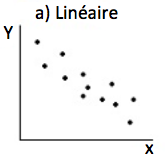
\includegraphics[width=3cm]{graphique_residus/lineaire1.png}




% je voulais faire un page récap de l'analyse des résidues mais je suis pas capable de mettre un graph dans le multi col
% % Analyses des résidus
% \newpage
% \section*{Analyse des résidus}
% L'analyse des résidus permet de valider les 4 postulats nécéssaires au modèle.

% \subsection*{Divers types de résidus}
% \begin{itemize}
% 	\item Les résidus ordinaires, $\varepsilon_i$ le ième résidu défini par $\varepsilon_i = Y_i - \hat{Y}_i$
% 	\begin{itemize}
% 		\item Si l'hypothèse $H_1$ est vrai: $E[\hat{\varepsilon}_i] = 0$
% 		\item Si l'hypothèse $H_2$ est vrai: $Var(\hat{\varepsilon}_i) = (1 - h_{ii})\sigma^2$ où $h_{ii} = 1/n + (x_i - \bar{x})^2 / S_{xx} $
% 		\item Si l'hypothèse $H_3$ est vrai: $cov(\hat{\varepsilon}_i, \hat{\varepsilon}_j) = -h_{ii}\sigma^2 $
% 		\item Si l'hypothèse $H_4$ est vrai: $\hat{\varepsilon}_i \sim N(0, (1 - h_{ii})\sigma^2)$
% 	\end{itemize}
% 	\item Les résidus studentisés, $r_i$ le ième résidu studentisés défini par
% 	\begin{align*}
% 		r_i = \frac{\hat{\varepsilon}_i}{s sqrt{1 - h_{ii}}}
% 	\end{align*}
% 	C'est résidues permet d'éliminer la non-homogénéité de la variance des risidue ordinaires et leur interprétation dans un graphique est beaucoup plus directe.
% \end{itemize}

% \subsection*{$H_1$: Linéarité}
% \begin{itemize}
% 	\item \textbf{Nuage de point de $Y_i$ en fonction $x_i$}
% 	\begin{figure}[!h]
% 		\centering
% 		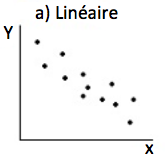
\includegraphics[width=3cm]{graphique_residus/lineaire1.png}
% 	 \end{figure}
% \end{itemize}







\end{multicols*}
%% -----------------------------
%% Fin du document
%% -----------------------------
\end{document}